\section{Introduction}

% the existence of influences by relations in dialogues
Interpersonal relationship is an implicit but important feature 
underlying all dialogues, shaping how language is used and perceived 
during communication. People start to practice such style shifting in 
communication at very early stage unconsciously. Study~\cite{mind-reading} 
finds that when children listen to another person, their understanding 
of the counterpart depends on nature of their relationship with the speaker. 
Study~\cite{conversational-motive} also find that conversations between 
different partners are executed under different interpersonal motives, 
and thus the dialogues differ in topics and styles. 
Also, similar expressions may reflect different emotions and attitudes in 
different relationships. 

% motivations of extract relationship between speaker 
Analyzing the relationship based on dialogues between interlocutors 
is well-motivated. First, it can provide dialogue systems with 
supplementary features for generating more suitable responses for different 
relationships, which helps in developing more intelligent role-playing chatbots.
Second, it is useful in recommendation systems if the system can figure 
out the relationship between users according to their privacy-insensitive chats.
Third, an automatic relationship classifier can help 
understand where the interpersonal stress/stimuli comes from in 
mental disorder treatment~\cite{tension-monitor,bopolar-monitor,cog-load}.
Besides, it can be also used for crime investigation, relieving
the burden of manual monitoring and improve the productivity of searching
in large amount of dialogue data. 

\begin{figure}[t!]
	\centering
	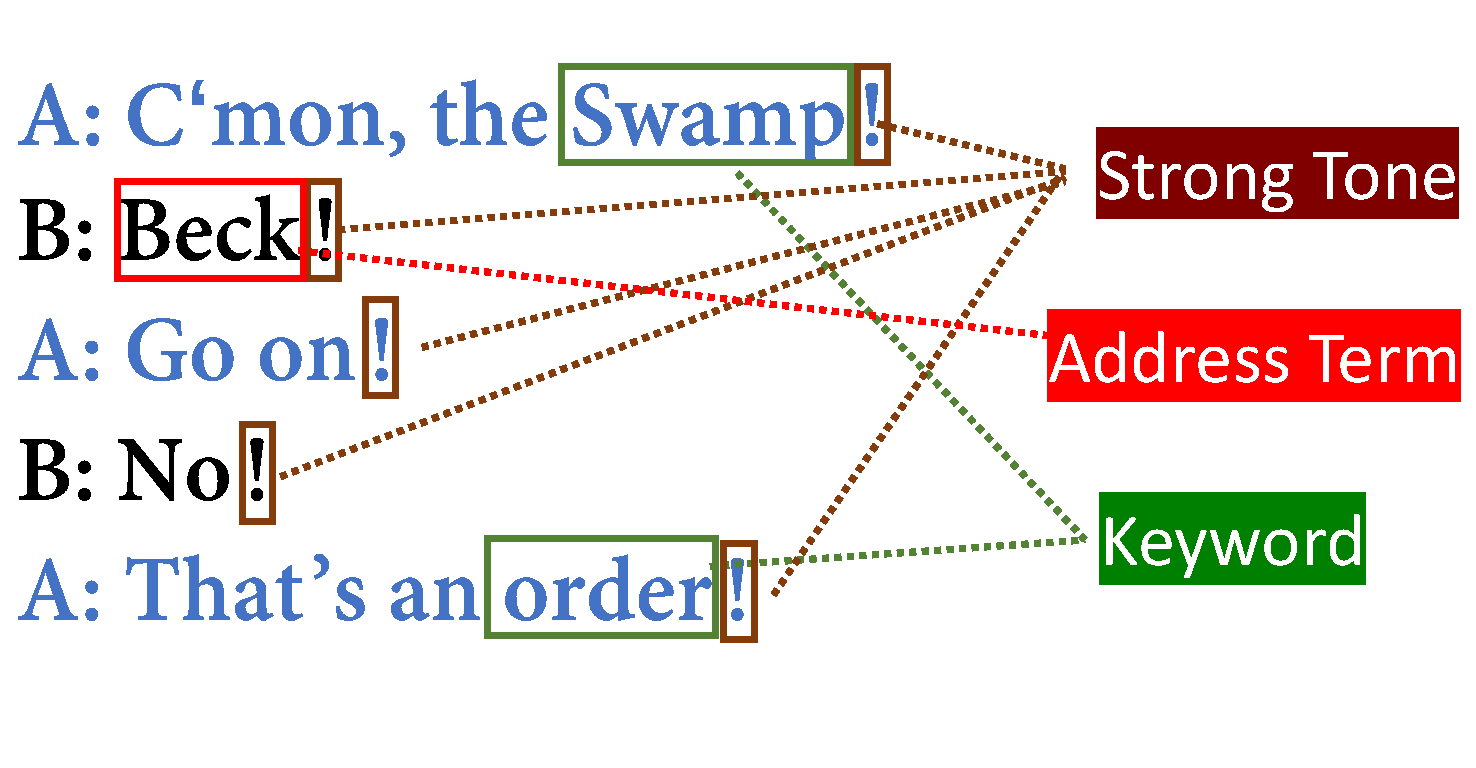
\includegraphics[width=0.85\columnwidth]{instinct.pdf}
	\caption{A sample dialogue and parts that are 
		reported as informative by human testers. }
	\label{fig:instinct}
\end{figure}

% challenges of this task
Relation classification of dialogue sessions is not an easy task. Figure \ref{fig:instinct} shows a 5-turn dialogue example. We can see that it's challenging to fully contextualize such short conversation without any prior knowledge, 
except one might infer that the two speakers are fellow soldiers 
in the military. Facing such problem, human usually resort to their 
communication experiences and commonsense knowledge to make sense of the background stories and give the inferences about the speakers' relationship. This shows that the inference of relationships from dialogues is possible but not straight forward for statistical models.

% the differences between previous datasets and ours
Previous work mainly focuses on relation classification between named entities. 
Sentence-level relation classification datasets, such as FewRel~\cite{HanZYWYLS18} and  TACRED~\cite{ZhangZCAM17}, have been widely studied~\cite{Zhang0M18,GaoH0S19,ZhangHLJSL19}, targeting on figuring out the correct relation type between entities within a given sentence. Recent research sets sights on the 
inter-sentence relations. DocRED~\cite{YaoYLHLLLHZS19} has been proposed 
as the largest document-level relation extraction dataset from plain text, 
where person (an entity type) only occupies 18.5\% of the entities. 
DialogRE~\cite{YuSCY20} aims at predicting the relations between two arguments 
in dialogues and MPDD~\cite{ChenHC20} is a Chinese dataset for predicting relations between speaker and listeners of each turn in a dialogue session.
However, relations in both datasets are limited to the current dialogue session, without cross-session considerations.


% introduction of our dataset
Different from their problem definition, we are trying to figure out the interpersonal 
relationships between speakers in dyadic dialogues from two perspectives, session-level and pair-level.
Multiple dialogue sessions may happen between each pair of speakers and 
it is usually not easy to figure out the relationship between 
a pair of speakers with only one session and no background context. 
Human has the ability to make the connections between multiple sessions 
and construct the whole picture between two speakers. 
In other words, cross-session inferences are required for final predictions. 

In this paper, we propose a new dyadic dialogue dataset for 
interpersonal relation classification called DDRel. 
The dataset consists of 6300 dialogue sessions from movie scripts crawled 
from IMSDb between 694 pair of speakers, annotated with relationship labels 
by human. 13 relation types according to 
Reis and Sprecher~\cite{reis2009encyclopedia} are covered in our dataset and these types can cover most of the interpersonal relations in daily life. 
Several strong baselines and human evaluations are implemented. 
The results and future work of our dataset are discussed.

% contributions
In summary, this paper makes following contributions:
\begin{itemize}
	\item We propose the task of dialogue relation classification for speakers, different from the previous intra-sentence or inter-sentence relation classification tasks (Sec.~\ref{sec:task}).
	\item To the best of our knowledge, we construct the first-ever dialogue relation classification dataset for analyzing interpersonal relationships between speakers with multiple dialogue sessions (Sec.~\ref{sec:dataset}). %\KZ{Is it really true now given MPDD?}
	\item We establish a set of classification baselines on our dataset using standard learning-based techniques. The gap between SOTA models and human performances show the difficulty of this task and higher requirements for current models (Sec.~\ref{experiments} and Sec.~\ref{sec:results}).
\end{itemize}
